\documentclass[tikz,border=4pt]{standalone}
\usepackage{mathptmx}
\usepackage{amsmath,amssymb}
\DeclareMathAlphabet{\mathcal}{OMS}{cmsy}{m}{n}
\usetikzlibrary{positioning,fit,decorations.pathmorphing,arrows.meta,calc,backgrounds}
\definecolor{ent}{HTML}{3B5B92}\definecolor{entfill}{HTML}{EEF2F9}
\definecolor{adv}{HTML}{B03A2E}\definecolor{advfill}{HTML}{FBEDEB}
\definecolor{trust}{HTML}{3E8E41}
\begin{document}
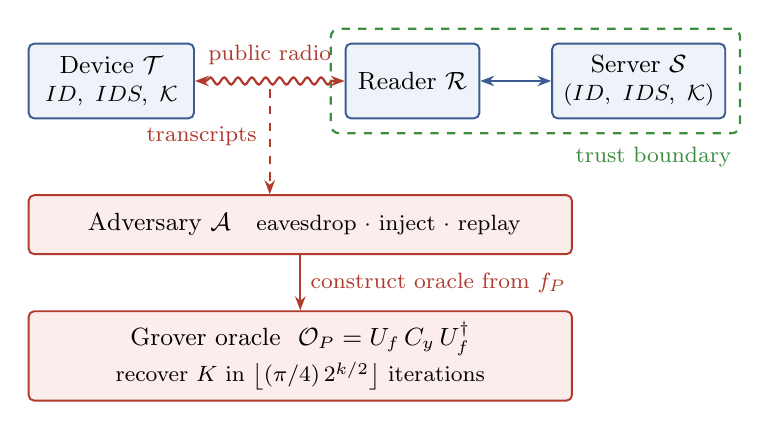
\begin{tikzpicture}[font=\small,
  box/.style={draw=ent,fill=entfill,rounded corners=2pt,line width=0.7pt,align=center,inner sep=4pt,minimum height=0.95cm},
  abox/.style={draw=adv,fill=advfill,rounded corners=2pt,line width=0.7pt,align=center,inner sep=4pt},
  >={Stealth[length=5pt]}]
\node[box,minimum width=2.1cm] (T) {Device $\mathcal{T}$\\[-1pt]{\footnotesize $ID,\ IDS,\ \mathcal{K}$}};
\node[box,minimum width=1.7cm,right=1.9cm of T] (R) {Reader $\mathcal{R}$};
\node[box,minimum width=2.1cm,right=0.9cm of R] (S) {Server $\mathcal{S}$\\[-1pt]{\footnotesize $(ID,\ IDS,\ \mathcal{K})$}};
\draw[<->,adv,line width=0.8pt,decorate,decoration={snake,amplitude=1.3pt,segment length=5pt,pre length=4pt,post length=4pt}] (T.east) -- node[above=2pt,font=\footnotesize,text=adv]{public radio} (R.west);
\draw[<->,ent,line width=0.8pt] (R.east) -- (S.west);
\begin{scope}[on background layer]
\node[draw=trust,dashed,line width=0.8pt,rounded corners=3pt,inner sep=5pt,fit=(R)(S)] (TB) {};
\end{scope}
\node[font=\footnotesize,text=trust,anchor=north east] at ([yshift=-1pt]TB.south east) {trust boundary};
\node[abox,anchor=north west,minimum width=6.9cm,minimum height=0.75cm] (A) at ([yshift=-0.95cm]T.south west) {\hspace{0.1cm}Adversary $\mathcal{A}$\quad{\footnotesize eavesdrop $\cdot$ inject $\cdot$ replay}};
\coordinate (mid) at ($(T.east)!0.5!(R.west)$);
\draw[->,adv,dashed,line width=0.8pt] ([yshift=-3pt]mid) -- (mid |- A.north) node[pos=0.45,left=1pt,font=\footnotesize,text=adv]{transcripts};
\node[abox,below=0.7cm of A,minimum width=6.9cm] (O) {Grover oracle\ \ $\mathcal{O}_P = U_f\, C_y\, U_f^{\dagger}$\\[1pt]{\footnotesize recover $K$ in $\big\lfloor (\pi/4)\,2^{k/2} \big\rfloor$ iterations}};
\draw[->,adv,line width=0.8pt] (A) -- node[right,font=\footnotesize,text=adv]{construct oracle from $f_P$} (O);
\end{tikzpicture}
\end{document}
